% ----------------------------------------------------------------------

\newpage

\subsection{\gainped Test}
\label{ss:gainped}

\subsubsection{Purpose}

The \gainped test does not alter any \dac parameters,
but merely evaluates the shape of the pulse height vs. \vcal distribution for each pixel.
For each pixel, th distribution is fitted and the fit parameters are stored for later use.
Since variations in gain are expected between pixels in a \roc,
the gain must be measured independantly for each pixel so that the pulse height to be calibrated back to the input signal size, 
in units of the \vcal~\dac (high range).

\subsubsection{\textcolor{red}{Methodology}}
\subsubsection{Output}

\begin{figure}[!Hp]
\centering
\begin{minipage}{0.45\textwidth}
  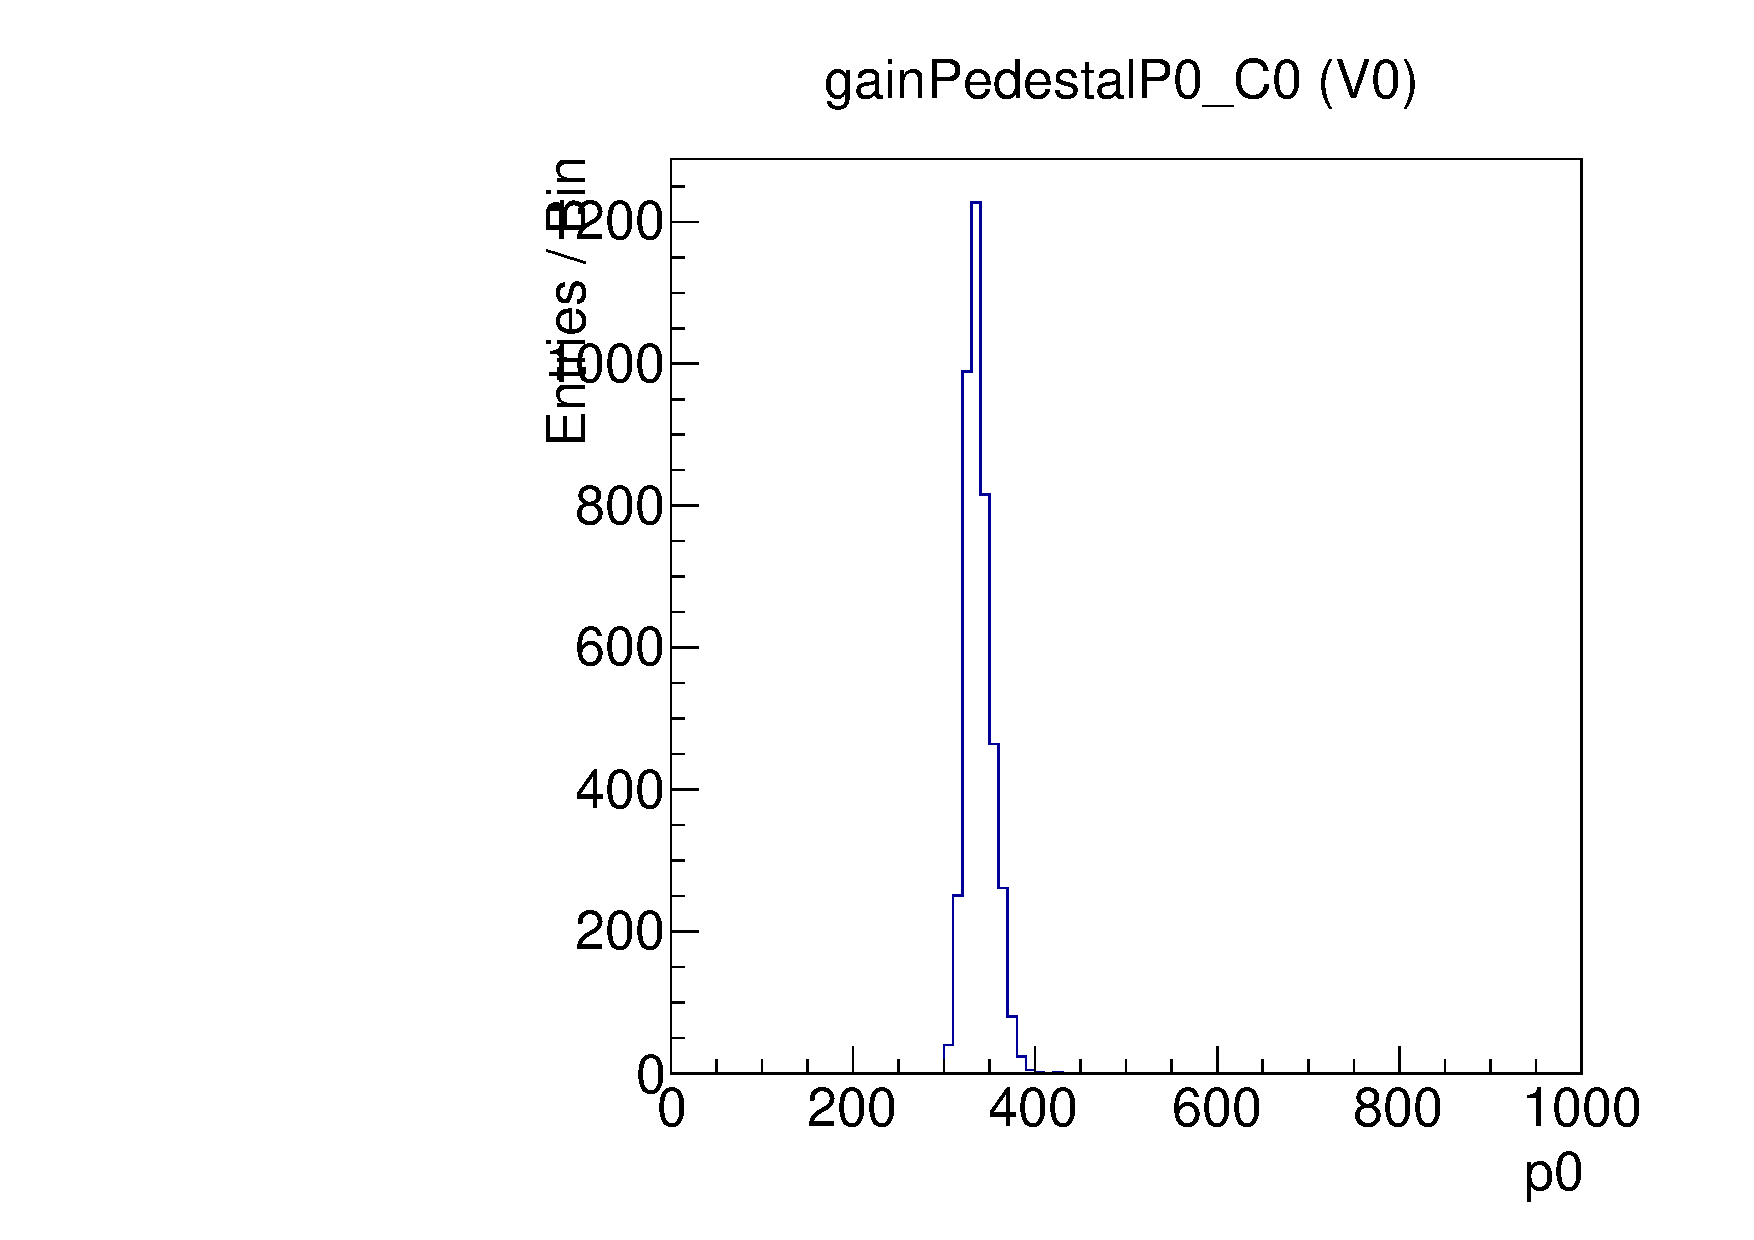
\includegraphics[width=1.0\textwidth]{figures/gainped_gainPedestalP0.pdf}
  \caption{}
  \label{fig:gainped_gainPedestalP0}
\end{minipage}
\hspace{0.3cm}
\begin{minipage}{0.45\textwidth}
  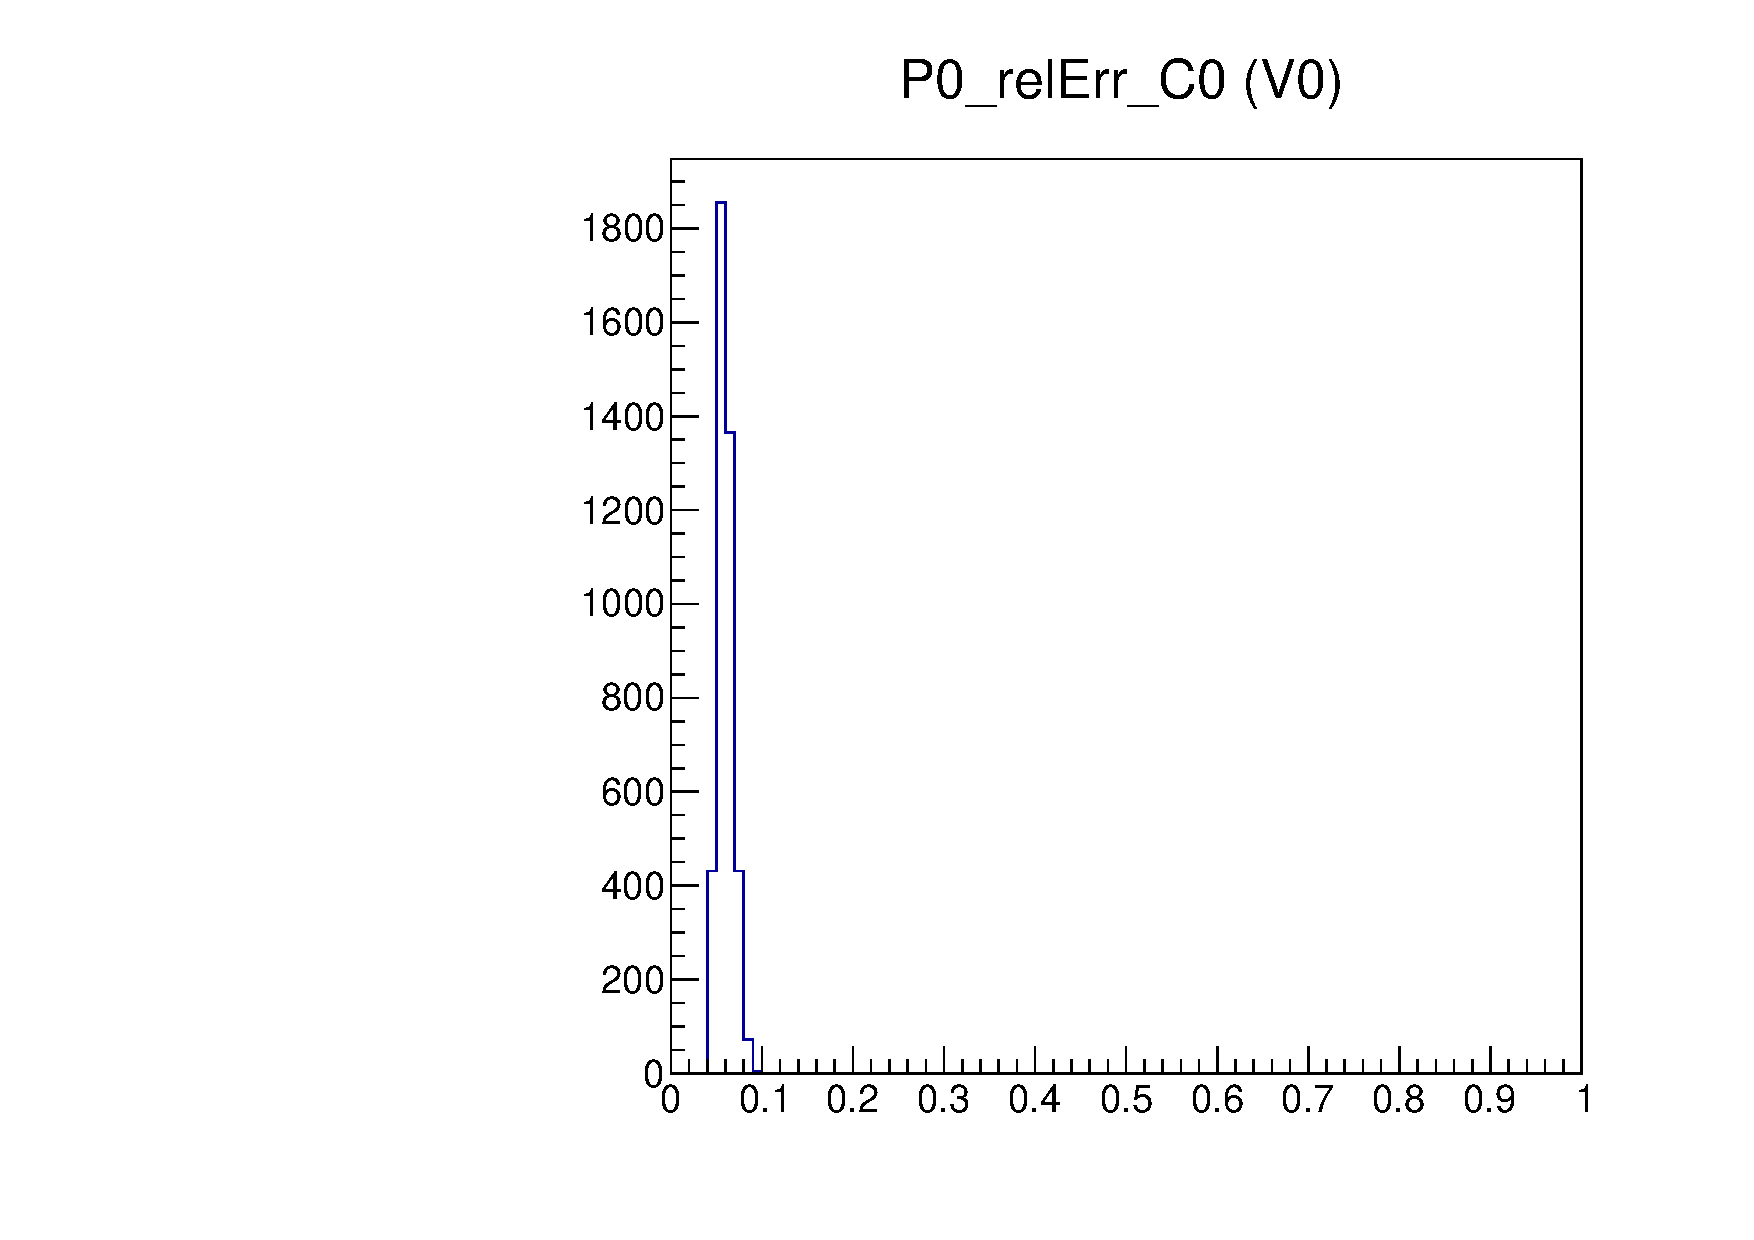
\includegraphics[width=1.0\textwidth]{figures/gainped_P0_relErr.pdf}
  \caption{}
  \label{fig:gainped_P0_relErr}
\end{minipage}
\end{figure}

\begin{figure}[!Hp]
\centering
\begin{minipage}{0.45\textwidth}
  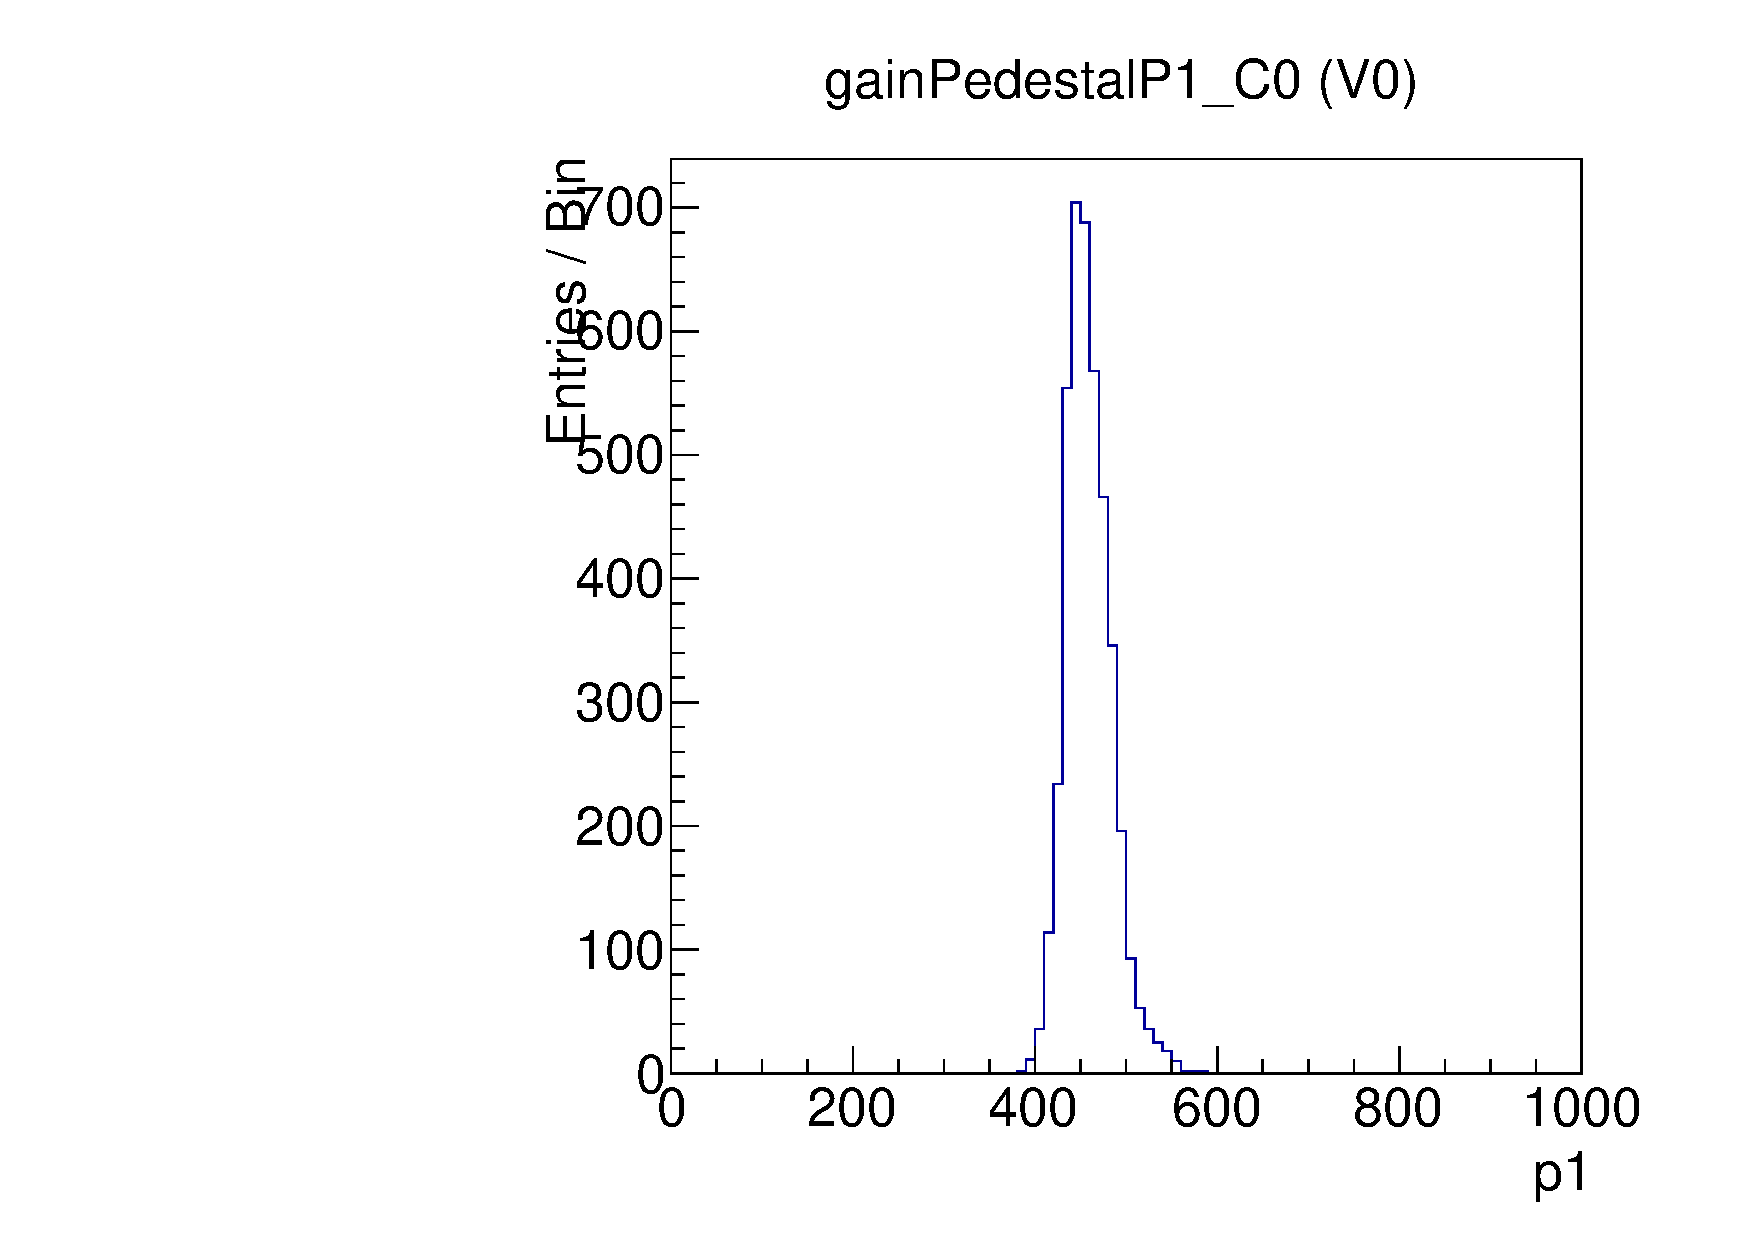
\includegraphics[width=1.0\textwidth]{figures/gainped_gainPedestalP1.pdf}
  \caption{}
  \label{fig:gainped_gainPedestalP1}
\end{minipage}
\hspace{0.3cm}
\begin{minipage}{0.45\textwidth}
  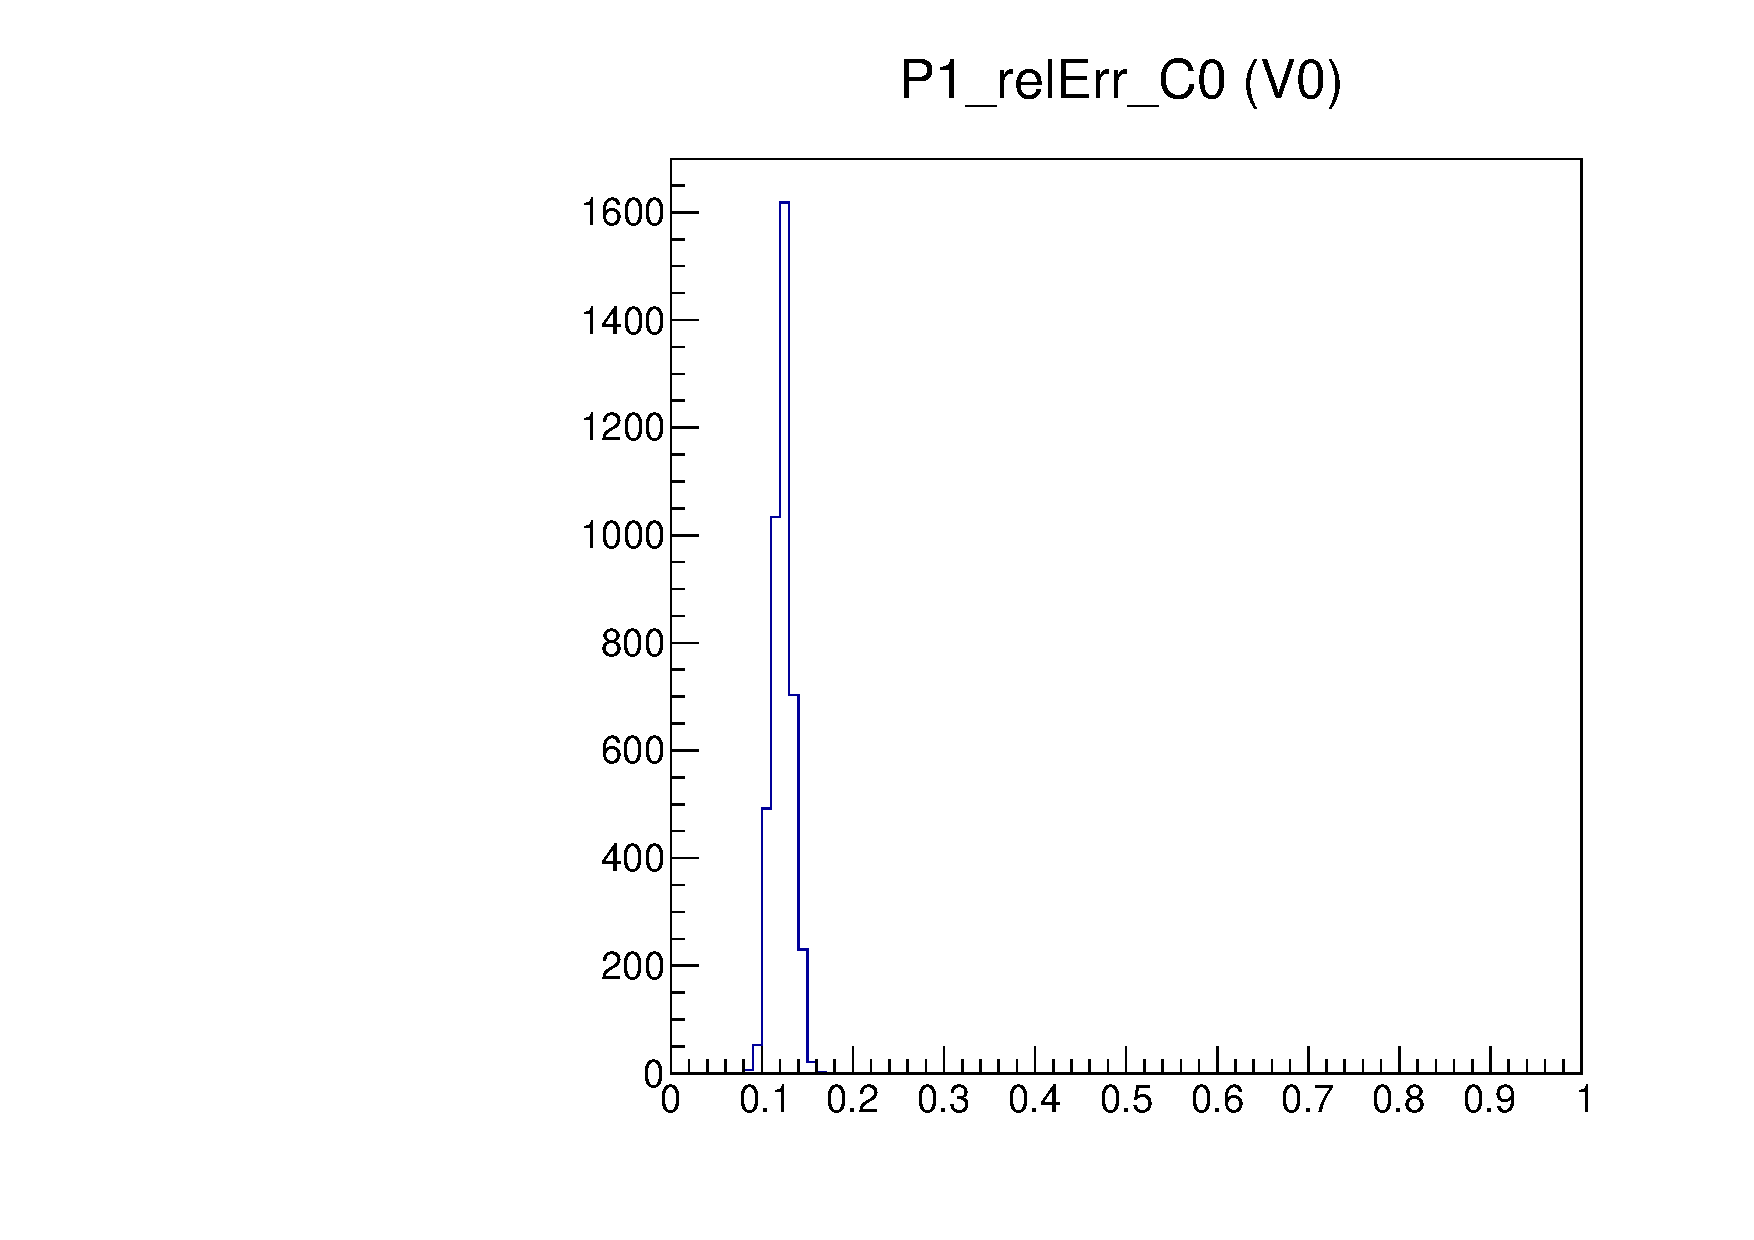
\includegraphics[width=1.0\textwidth]{figures/gainped_P1_relErr.pdf}
  \caption{}
  \label{fig:gainped_P1_relErr}
\end{minipage}
\end{figure}

\begin{figure}[!Hp]
\centering
\begin{minipage}{0.45\textwidth}
  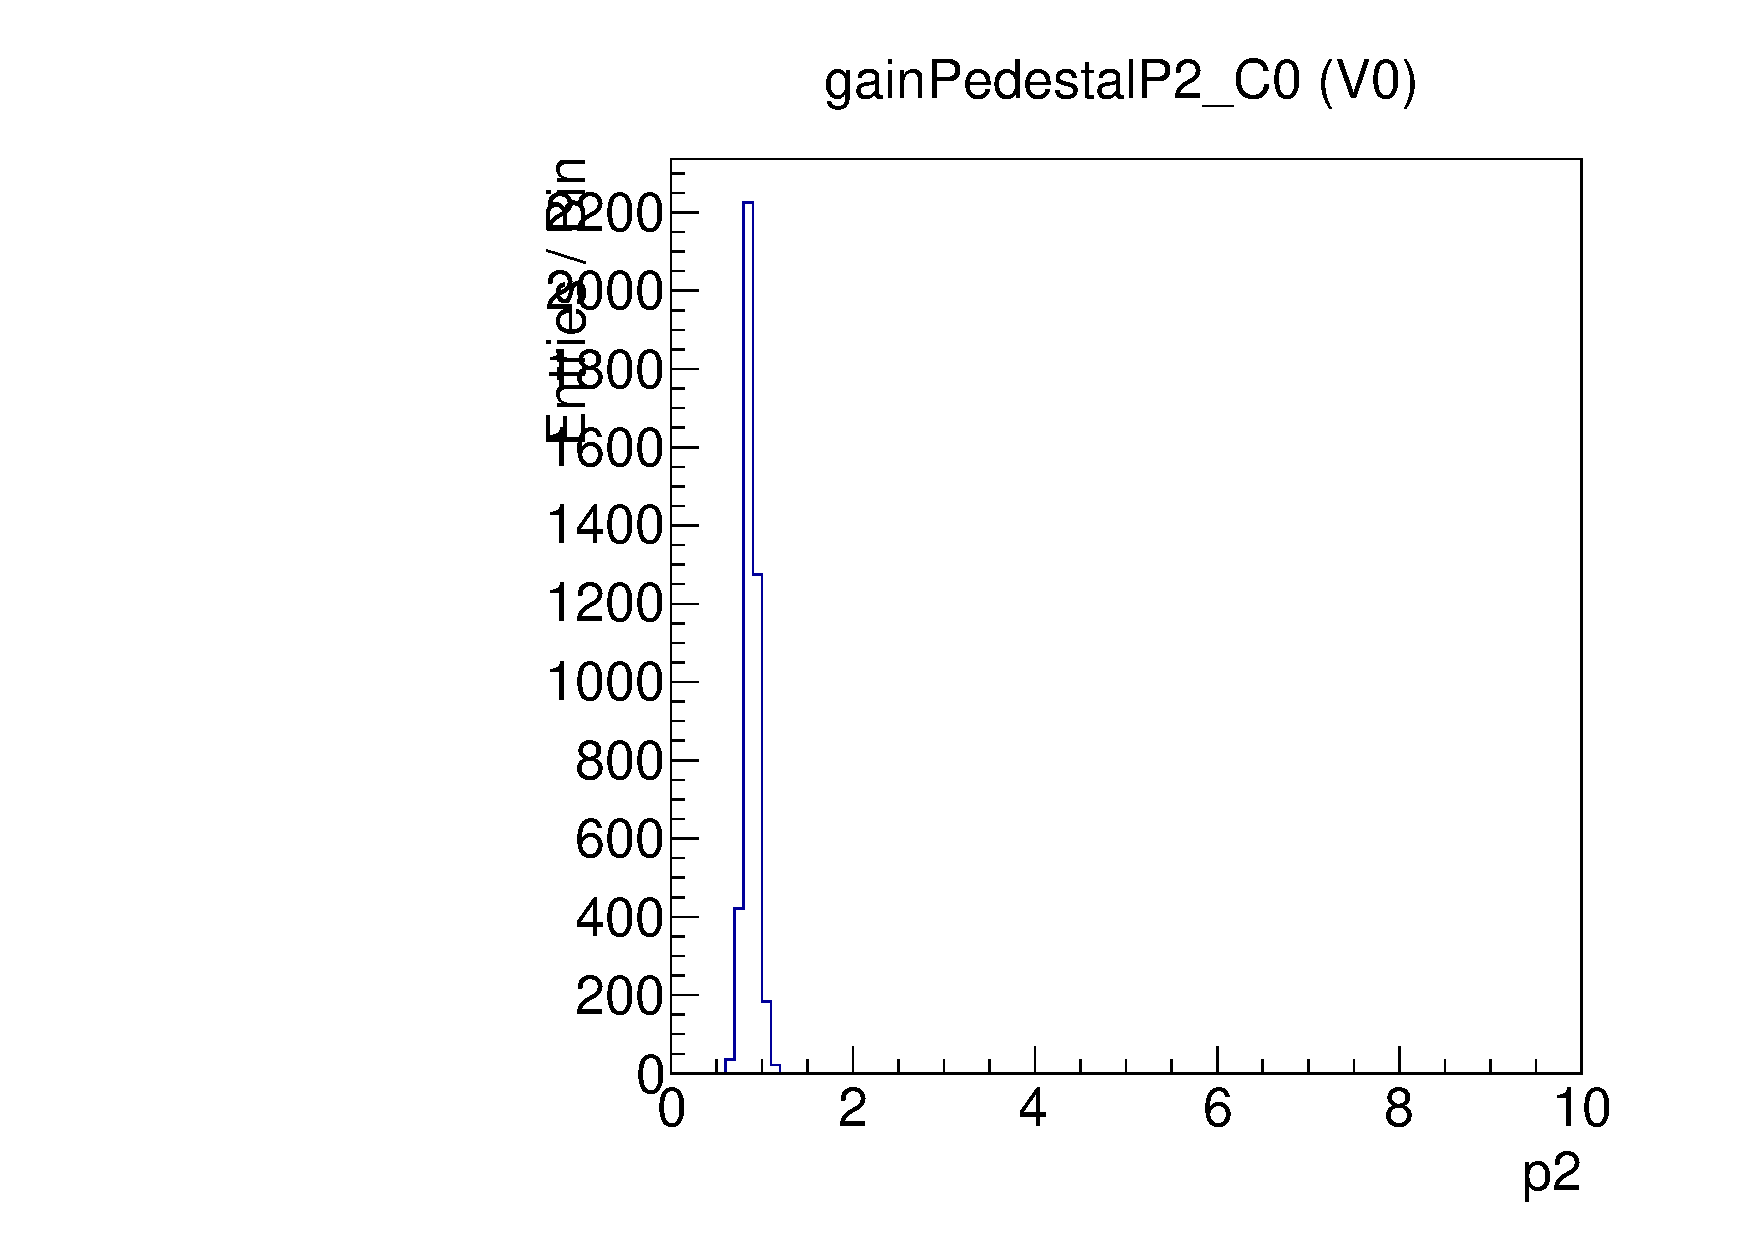
\includegraphics[width=1.0\textwidth]{figures/gainped_gainPedestalP2.pdf}
  \caption{}
  \label{fig:gainped_gainPedestalP2}
\end{minipage}
\hspace{0.3cm}
\begin{minipage}{0.45\textwidth}
  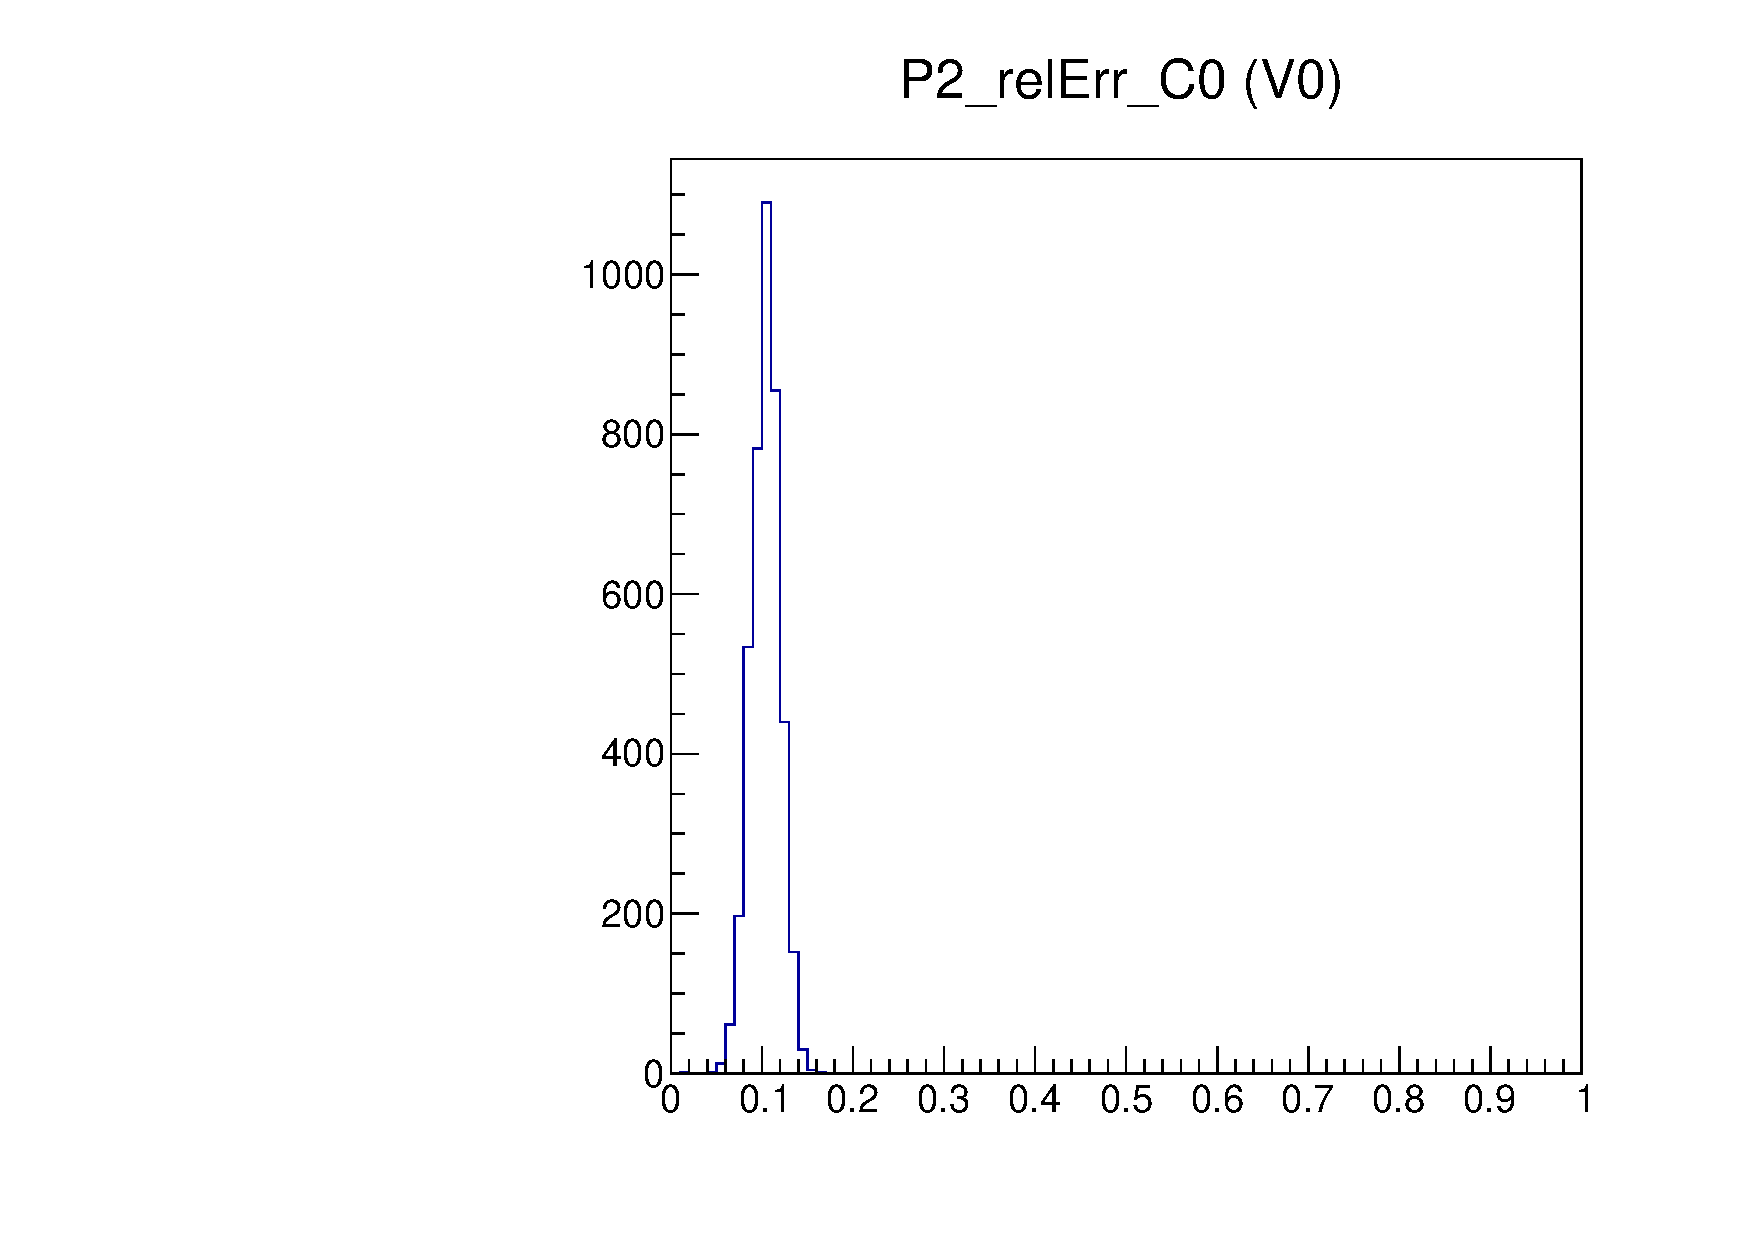
\includegraphics[width=1.0\textwidth]{figures/gainped_P2_relErr.pdf}
  \caption{}
  \label{fig:gainped_P2_relErr}
\end{minipage}
\end{figure}

\begin{figure}[!Hp]
\centering
\begin{minipage}{0.45\textwidth}
  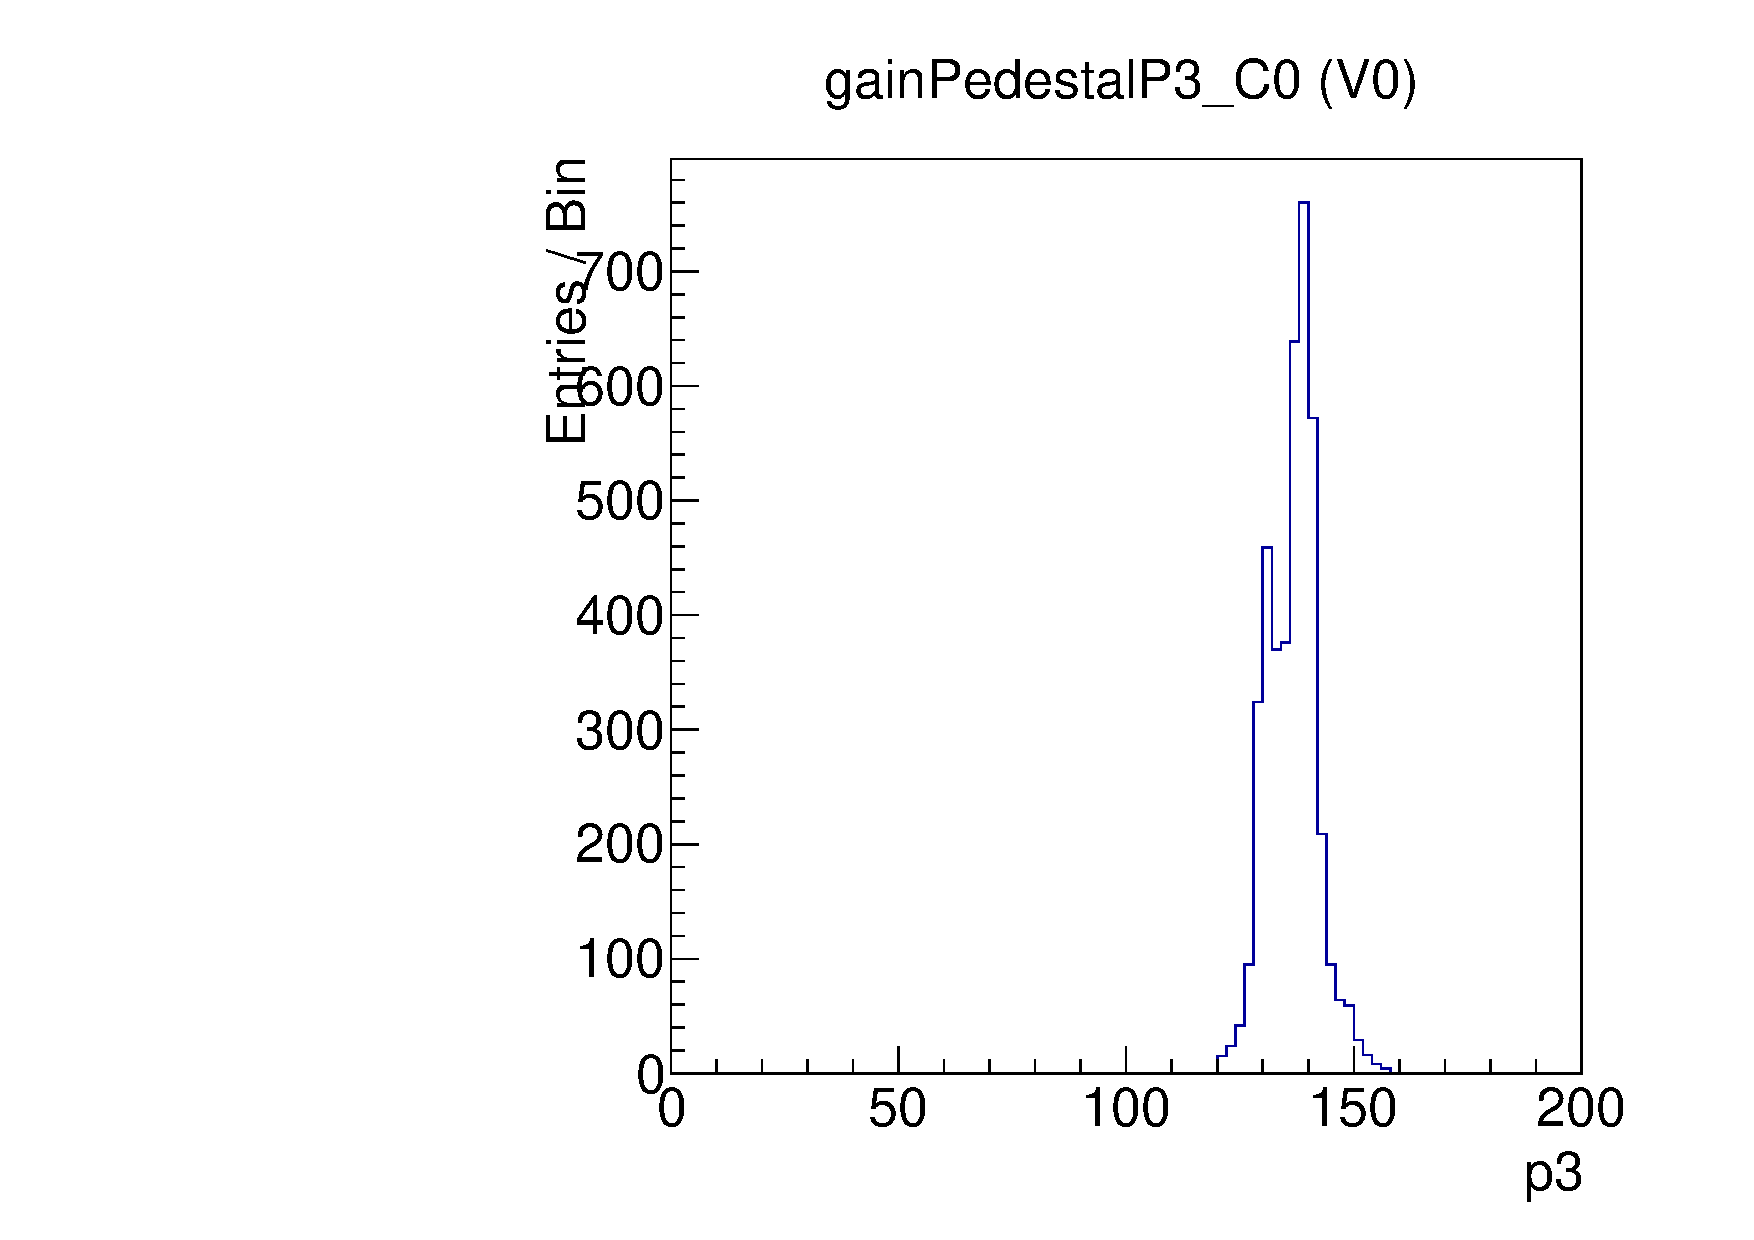
\includegraphics[width=1.0\textwidth]{figures/gainped_gainPedestalP3.pdf}
  \caption{}
  \label{fig:gainped_gainPedestalP3}
\end{minipage}
\hspace{0.3cm}
\begin{minipage}{0.45\textwidth}
  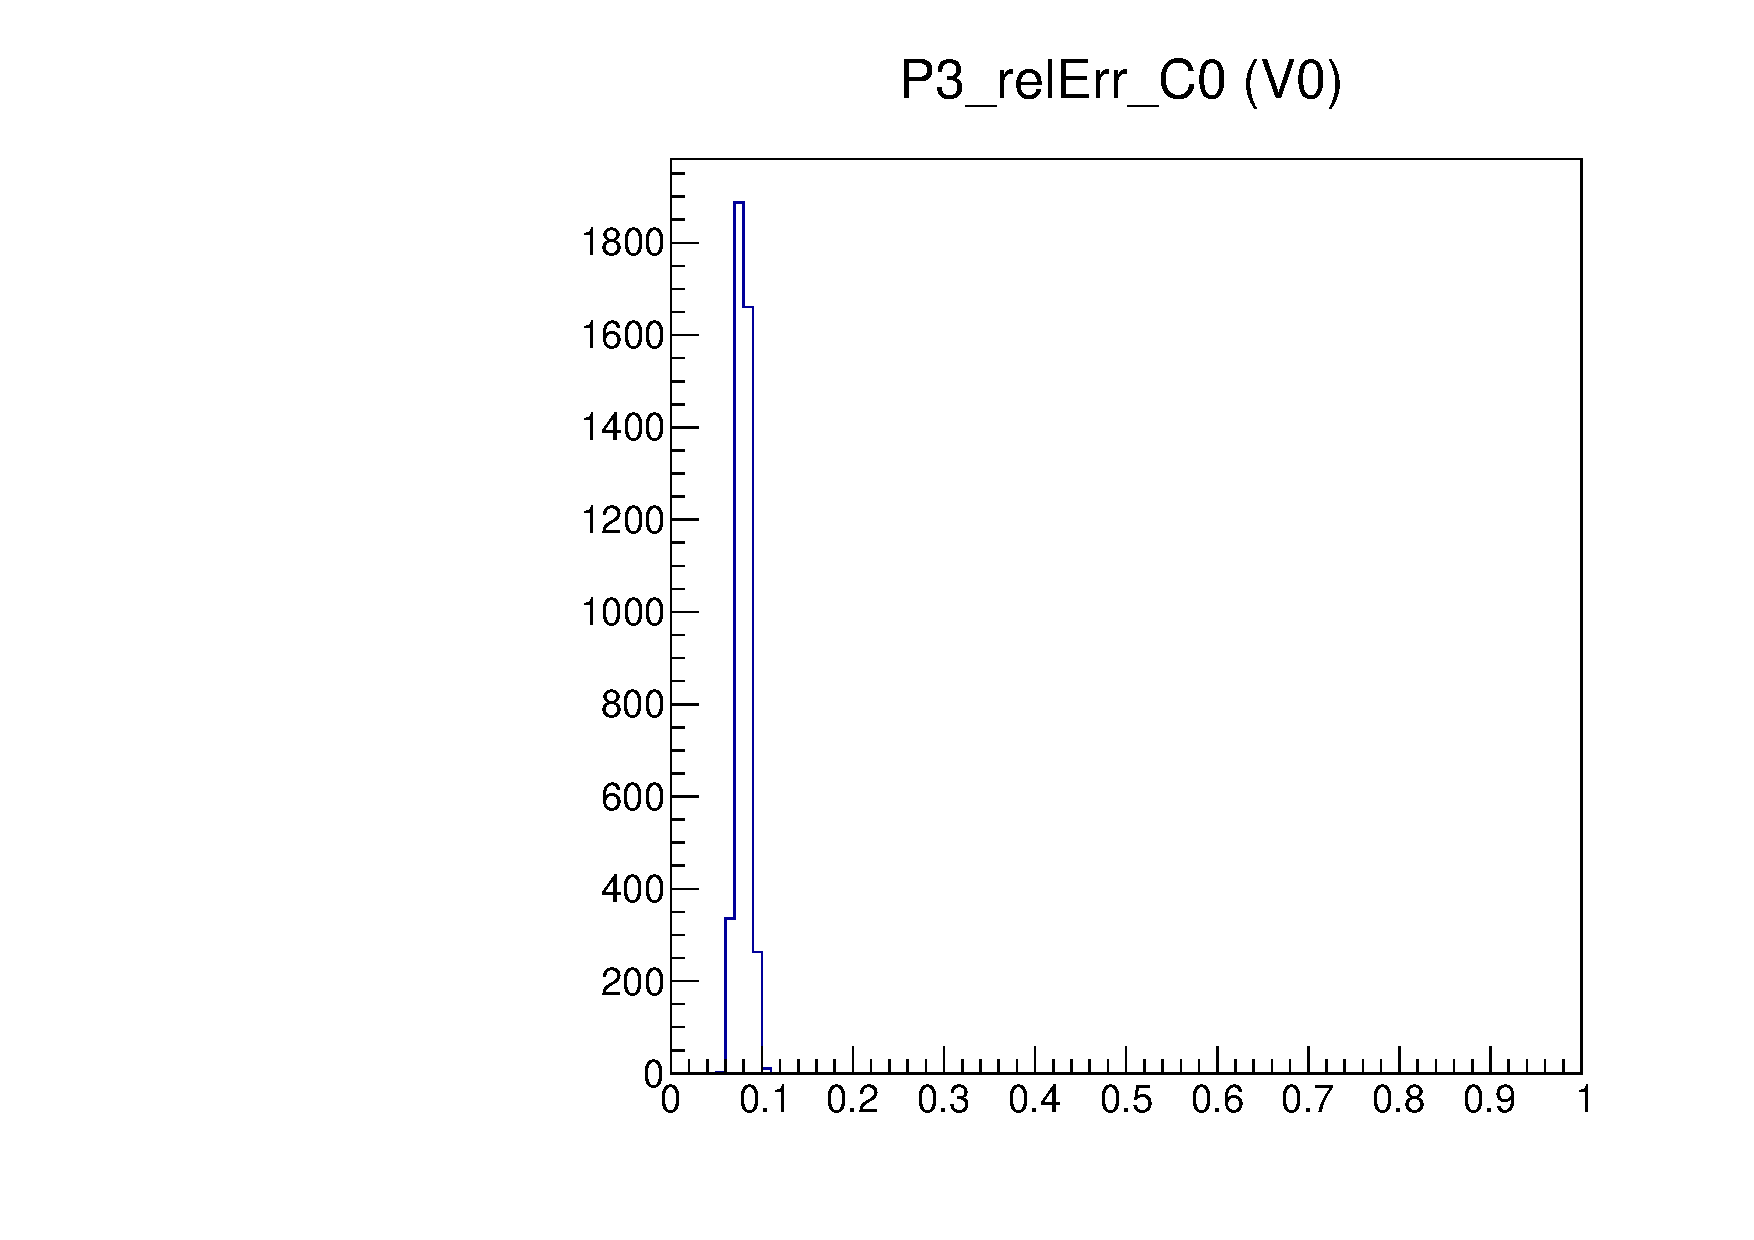
\includegraphics[width=1.0\textwidth]{figures/gainped_P3_relErr.pdf}
  \caption{}
  \label{fig:gainped_P3_relErr}
\end{minipage}
\end{figure}

\begin{figure}[!Hp]
\centering
\begin{minipage}{0.45\textwidth}
  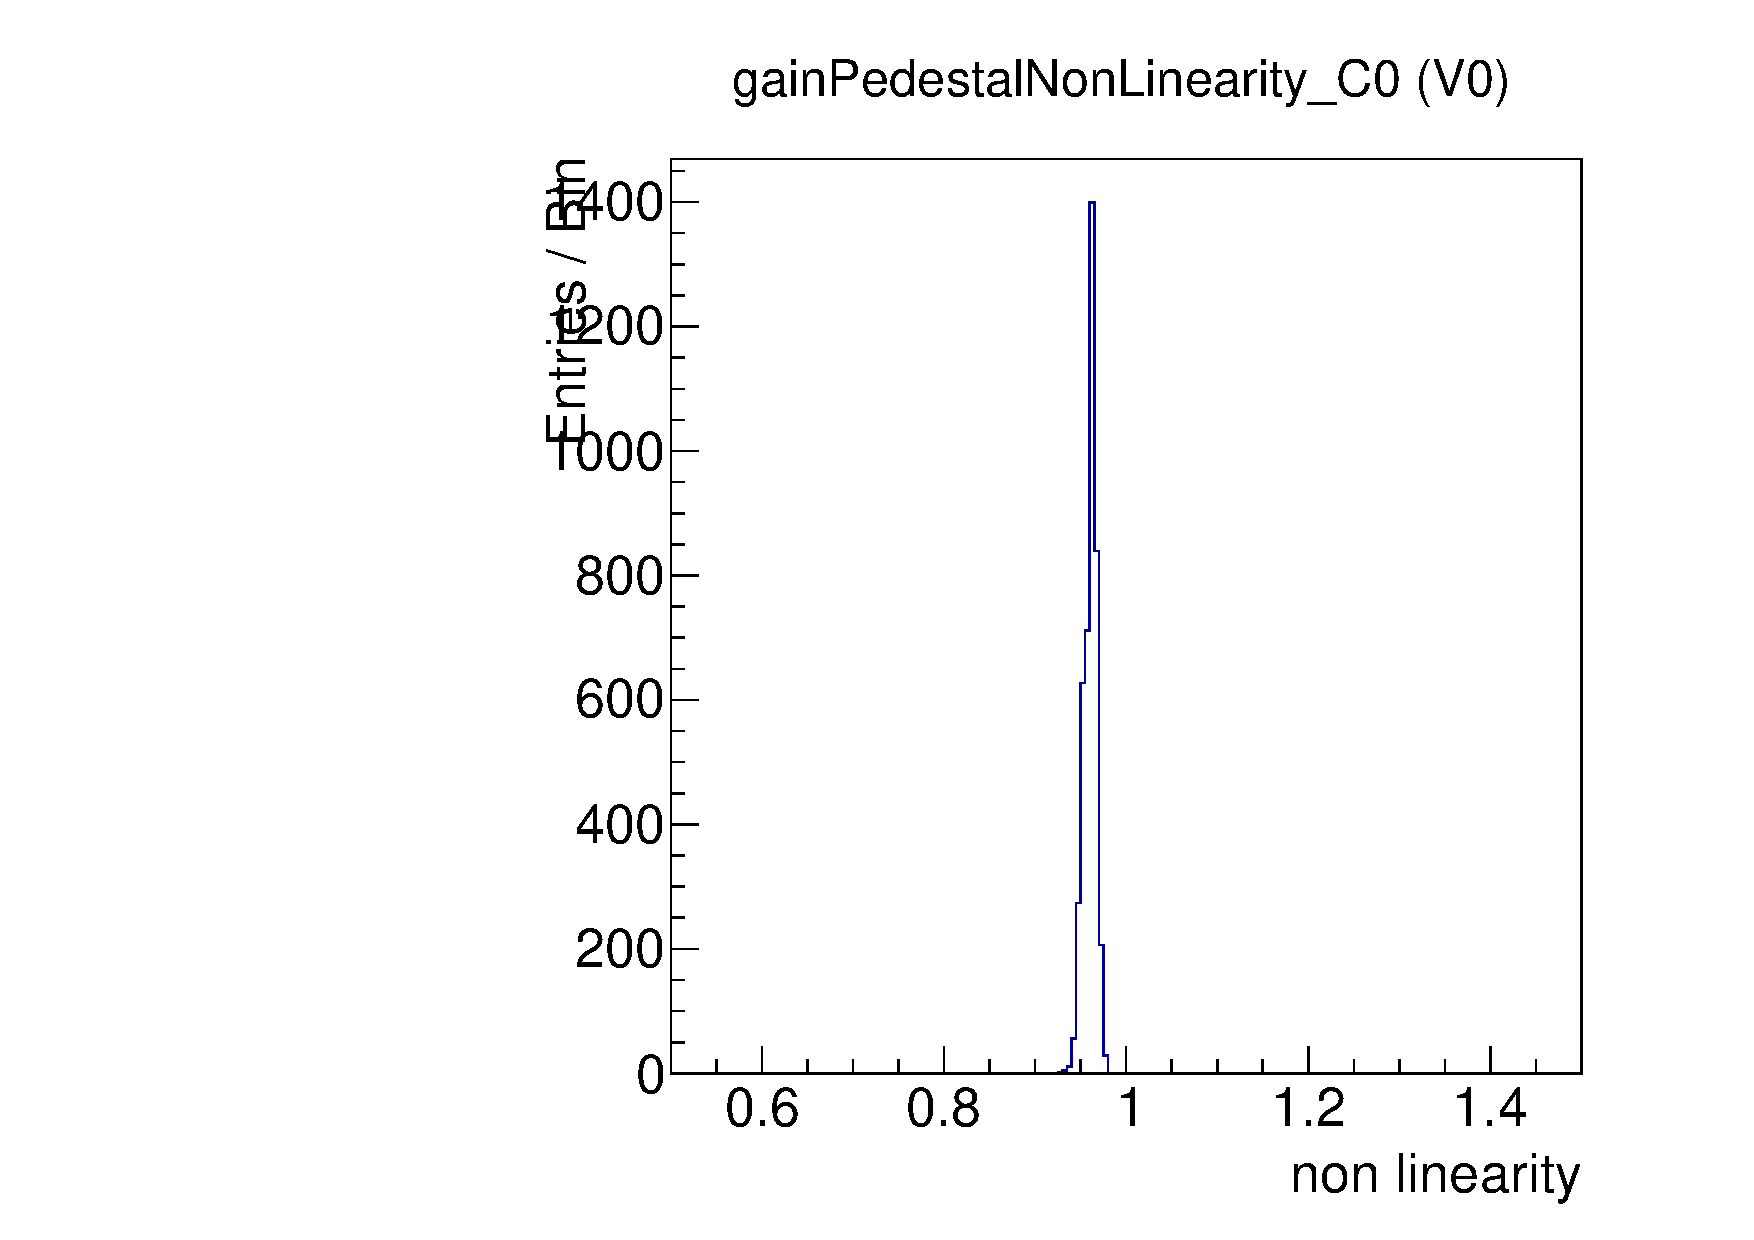
\includegraphics[width=1.0\textwidth]{figures/gainped_gainPedestalNonLinearity.pdf}
  \caption{}
  \label{fig:gainped_gainPedestalNonLinearity}
\end{minipage}
\end{figure}
